\documentclass[12pt,a4paper]{report}
\usepackage[utf8]{inputenc}
\usepackage[spanish]{babel}
\usepackage{geometry}
\usepackage{graphicx}
\usepackage{fancyhdr}
\usepackage{titlesec}
\usepackage{listings}
\usepackage{xcolor}
\usepackage{hyperref}
\usepackage{amsmath}
\usepackage{amssymb}
\usepackage{enumitem}
\usepackage{booktabs}
\usepackage{array}
\usepackage{longtable}

% Configuración de página
\geometry{margin=2.5cm}
\pagestyle{fancy}
\fancyhf{}
\fancyhead[L]{\leftmark}
\fancyhead[R]{\thepage}
\renewcommand{\headrulewidth}{0.4pt}

% Configuración de código
\definecolor{codegreen}{rgb}{0,0.6,0}
\definecolor{codegray}{rgb}{0.5,0.5,0.5}
\definecolor{codepurple}{rgb}{0.58,0,0.82}
\definecolor{backcolour}{rgb}{0.95,0.95,0.92}

\lstdefinestyle{mystyle}{
    backgroundcolor=\color{backcolour},   
    commentstyle=\color{codegreen},
    keywordstyle=\color{magenta},
    numberstyle=\tiny\color{codegray},
    stringstyle=\color{codepurple},
    basicstyle=\ttfamily\footnotesize,
    breakatwhitespace=false,         
    breaklines=true,                 
    captionpos=b,                    
    keepspaces=true,                 
    numbers=left,                    
    numbersep=5pt,                  
    showspaces=false,                
    showstringspaces=false,
    showtabs=false,                  
    tabsize=2
}

\lstset{style=mystyle}

% Configuración de títulos
\titleformat{\chapter}[display]
  {\normalfont\huge\bfseries}{\chaptertitlename\ \thechapter}{20pt}{\Huge}
\titlespacing*{\chapter}{0pt}{50pt}{40pt}

% Configuración de hipervínculos
\hypersetup{
    colorlinks=true,
    linkcolor=blue,
    filecolor=magenta,      
    urlcolor=cyan,
    pdftitle={Manual Técnico - Sistema de Generación de Exámenes con IA},
    pdfauthor={Equipo de Desarrollo},
}

\begin{document}

% Página de título
\begin{titlepage}
    \centering
    \vspace*{2cm}
    
    {\Huge\bfseries MANUAL TÉCNICO}\\[0.5cm]
    {\Large TODO SOBRE EL DESARROLLO DE LA APLICACIÓN}\\[2cm]
    
    {\Huge\bfseries ExamGenAI}\\[0.5cm]
    {\Large Sistema de Generación de Exámenes con IA}\\[3cm]
    
    {\large\bfseries DESARROLLADA POR:}\\[0.5cm]
    {\large HERNÁNDEZ TELLEZ HÉCTOR FIDEL}\\
    {\large RIVERO FLORES VICTOR GABRIEL  }\\
    
    {\large Versión 1.0}\\[0.5cm]
    {\large 19 de junio de 2025}\\[2cm]
    
    {\large Desarrollado con React, Node.js y Flutter}\\
    {\large Integración con Supabase y Google Gemini AI}
    
    \vfill
\end{titlepage}

% Tabla de contenidos
\tableofcontents
\newpage

\chapter{Introducción}

\section{Tecnologías}

El Sistema de Generación de Exámenes con IA (ExamGenAI) es una plataforma web moderna diseñada para automatizar la creación de exámenes personalizados utilizando inteligencia artificial. El sistema permite a los usuarios subir documentos, generar preguntas automáticamente, realizar exámenes con temporizador y recibir retroalimentación detallada.

\subsection{Stack Tecnológico Detallado}

\subsubsection{Frontend}
\begin{itemize}
    \item \textbf{React 19.0.0}: Framework principal para la interfaz de usuario
    \item \textbf{TypeScript}: Lenguaje de programacion con tipado estático
    \item \textbf{Vite}: Herramienta de build rápida y servidor de desarrollo
    \item \textbf{Tailwind CSS}: Framework de CSS para diseño responsive
    \item \textbf{React Router}: Librería de enrutamiento para SPA
    \item \textbf{Motion}: Librería de animaciones para React
    \item \textbf{SweetAlert2}: Librería para alertas y modales elegantes
    \item \textbf{React Markdown}: Renderizador de contenido Markdown
    \item \textbf{KaTeX}: Renderizador de fórmulas matemáticas
\end{itemize}

\subsubsection{Backend}
\begin{itemize}
    \item \textbf{Node.js}: Runtime de JavaScript del lado del servidor
    \item \textbf{Express.js}: Framework web minimalista y flexible
    \item \textbf{Google Generative AI}: Integración con Gemini AI
    \item \textbf{Multer}: Middleware para manejo de archivos multipart
    \item \textbf{CORS}: Middleware para habilitar cross-origin requests
    \item \textbf{dotenv}: Gestión de variables de entorno
\end{itemize}

\subsubsection{Base de Datos y Servicios}
\begin{itemize}
    \item \textbf{Supabase}: Plataforma Backend-as-a-Service (PostgreSQL)
    \item \textbf{Google Gemini AI}: Servicio de inteligencia artificial
    \item \textbf{Hostinger}: Plataforma de hosting para el frontend
\end{itemize}

% --- NUEVA SECCIÓN ---
\subsubsection{Cliente Móvil (Wrapper)}
\begin{itemize}
    \item \textbf{Flutter}: Framework para el desarrollo de aplicaciones móviles multiplataforma.
    \item \textbf{webview\_flutter}: Paquete para integrar una vista web (WebView) dentro de la aplicación Flutter, permitiendo mostrar la aplicación web de React como si fuera una aplicación nativa.
\end{itemize}
% --- FIN DE NUEVA SECCIÓN ---

\chapter{Arquitectura del Sistema}

\section{Patrón Arquitectónico}

El sistema ExamGenAI sigue una arquitectura de tres capas bien definidas, separando las responsabilidades entre presentación, lógica de negocio y acceso a datos.

\begin{figure}[h]
\centering
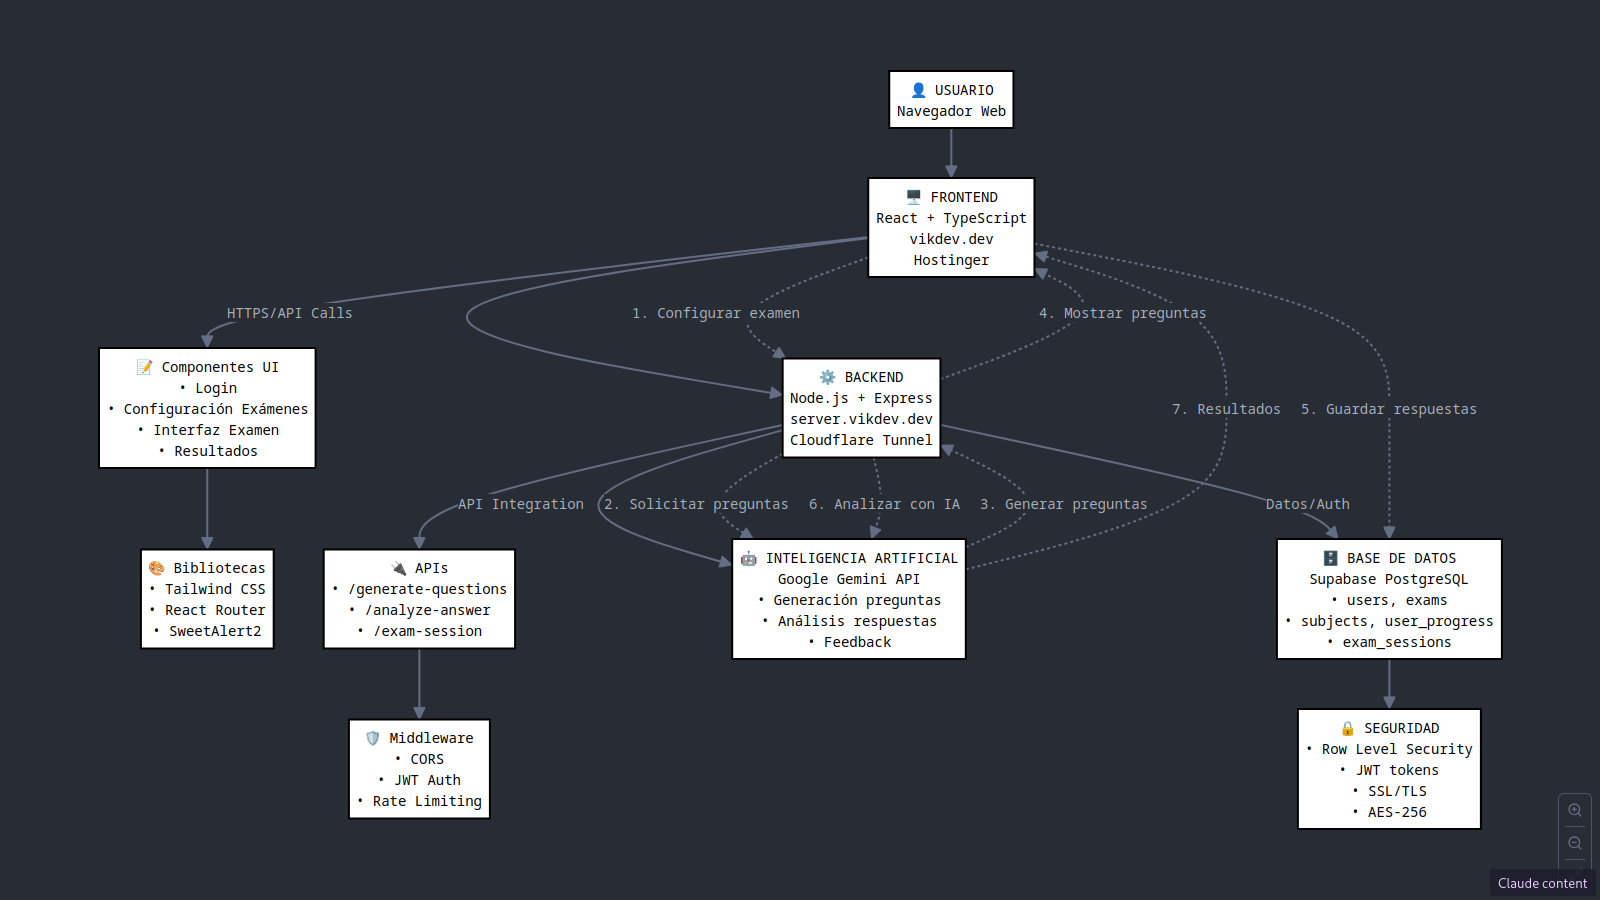
\includegraphics[width=0.9\textwidth]{arquitectura_sistema.png}
\caption{Diagrama de Arquitectura del Sistema ExamGenAI}
\label{fig:arquitectura}
\end{figure}


\subsection{Capas de la Arquitectura}

\subsubsection{Capa de Presentación (Frontend)}
\begin{itemize}
    \item \textbf{Componentes React}: Elementos de interfaz reutilizables
    \item \textbf{Páginas}: Vistas principales de la aplicación
    \item \textbf{Context API}: Gestión de estado global
    \item \textbf{Hooks personalizados}: Lógica reutilizable
\end{itemize}

% --- NUEVA SECCIÓN ---
\subsubsection{Cliente Móvil (Wrapper con Flutter)}
Adicionalmente, se ha desarrollado un \textit{wrapper} o contenedor móvil utilizando Flutter. Esta capa no contiene lógica de negocio, sino que su única función es encapsular la aplicación web de React (Capa de Presentación) dentro de una WebView. Esto permite distribuir la aplicación en tiendas de aplicaciones móviles y ofrecer una experiencia de usuario más integrada en dispositivos móviles, aprovechando el 100\% del código y funcionalidades ya desarrolladas para la web.
% --- FIN DE NUEVA SECCIÓN ---

\subsubsection{Capa de Lógica de Negocio (Backend)}
\begin{itemize}
    \item \textbf{API REST}: Endpoints para operaciones CRUD
    \item \textbf{Middleware}: Autenticación y validación
    \item \textbf{Servicios}: Integración con APIs externas
    \item \textbf{Controladores}: Manejo de la lógica de aplicación
\end{itemize}

\subsubsection{Capa de Datos}
\begin{itemize}
    \item \textbf{Supabase}: Base de datos PostgreSQL
    \item \textbf{Autenticación}: Sistema de usuarios integrado
    \item \textbf{Storage}: Almacenamiento de archivos
    \item \textbf{Real-time}: Actualizaciones en tiempo real
\end{itemize}

\subsection{Estructura de Directorios}

\subsubsection{Frontend}
\begin{lstlisting}
frontend/
+-- src/
    +-- API/
        +-- Gemini.tsx         # Configuracion API Gemini
    +-- components/
        +-- Main/              # Componentes principales
        +-- Examen/            # Componentes de examenes
        +-- Navbar.tsx         # Barra de navegacion
    +-- context/
        +-- AuthContext.tsx    # Context de autenticacion
    +-- pages/
        +-- Login.tsx          # Pagina de login
        +-- Examenes.tsx       # Pagina de examenes
        +-- Dashboard.tsx      # Panel principal
    +-- routers/
        +-- routes.tsx         # Configuracion de rutas
    +-- utils/                 # Utilidades
    +-- styles/                # Estilos globales
\end{lstlisting}

\subsubsection{Backend}
\begin{lstlisting}
backend/
+-- src/
    +-- index.js              # Servidor principal
    +-- reqAuthMiddleware.js  # Middleware de autenticacion
    +-- reqSupabase.js        # Integracion con Supabase
    +-- local.js              # Configuracion local
    +-- analize.js            # Analisis de documentos
    +-- routes/               # Rutas de la API
    +-- services/             # Servicios externos
    +-- utils/                # Utilidades del servidor
+-- uploads/                  # Archivos temporales
+-- package.json              # Dependencias
\end{lstlisting}

\section{Gestión de Estado}

\subsection{Context API de React}

El sistema utiliza React Context API para manejar el estado global de la aplicación, especialmente para:

\begin{itemize}
    \item \textbf{Autenticación}: Estado del usuario y sesión
    \item \textbf{Datos de examenes}: Información de examenes activos
    \item \textbf{Configuración}: Preferencias del usuario
    \item \textbf{Notificaciones}: Sistema de mensajes y alertas
\end{itemize}

\subsection{Providers Principales}

\subsubsection{AuthProvider}
\begin{lstlisting}
// Manejo de autenticacion y sesion de usuario
export const AuthProvider = ({ children }) => {
  const [user, setUser] = useState(null);
  const [loading, setLoading] = useState(true);
  
  // Metodos de login, logout, registro
  const login = async (email, password) => { ... };
  const logout = async () => { ... };
  const register = async (userData) => { ... };
  
  return (
    <AuthContext.Provider value={{
      user, login, logout, register, loading
    }}>
      {children}
    </AuthContext.Provider>
  );
};
\end{lstlisting}

\section{Componentes Principales}

\subsection{Integración con Gemini AI}

El sistema integra Google Gemini AI para la generación automática de contenido educativo:

\subsubsection{Configuración del Modelo}
\begin{lstlisting}
import { GoogleGenerativeAI } from "@google/generative-ai";

const genAI = new GoogleGenerativeAI(process.env.GEMINI_API_KEY);

// Configuracion para examenes faciles
const model_flash = genAI.getGenerativeModel({
  model: "gemini-2.0-flash"
});

// Configuracion para examenes complejos
const model_pro = genAI.getGenerativeModel({
  model: "gemini-2.5-pro-exp-03-25"
});
\end{lstlisting}

\subsubsection{Funcionalidades de IA}
\begin{itemize}
    \item \textbf{Generación de preguntas}: A partir de documentos subidos
    \item \textbf{Análisis de contenido}: Extracción de conceptos clave
    \item \textbf{Retroalimentación personalizada}: Explicaciones detalladas
    \item \textbf{Adaptación de dificultad}: Ajuste automático del nivel
\end{itemize}

\subsection{Sistema de Autenticación}

\subsubsection{Flujo de Autenticación}
\begin{enumerate}
    \item Usuario ingresa credenciales
    \item Validación con Supabase Auth
    \item Generación de JWT token
    \item Almacenamiento seguro en localStorage
    \item Protección de rutas privadas
\end{enumerate}

\begin{figure}[h]
\centering

\includegraphics[width=0.8\textwidth]{login_pantalla.png}
\caption{Pantalla de Login del Sistema ExamGenAI}
\label{fig:login}
\end{figure}


\subsubsection{Middleware de Seguridad}
\begin{lstlisting}
// Middleware para verificar autenticacion
export const getUserFromRequest = async (req) => {
  const token = req.headers.authorization?.split(' ')[1];
  
  if (!token) {
    throw new Error('Token no proporcionado');
  }
  
  const { data: user, error } = await supabase.auth.getUser(token);
  
  if (error || !user) {
    throw new Error('Token invalido');
  }
  
  return user;
};
\end{lstlisting}

\chapter{Pantallas y Funcionalidades}

\section{Dashboard Principal}

El dashboard es la pantalla principal después del login, proporcionando una vista general del sistema:

\subsection{Componentes del Dashboard}
\begin{itemize}
    \item \textbf{Panel de estadísticas}: Resumen de examenes realizados
    \item \textbf{Examenes recientes}: Lista de examenes completados
    \item \textbf{Accesos rápidos}: Botones para funciones principales
    \item \textbf{Notificaciones}: Mensajes y actualizaciones del sistema
\end{itemize}

\subsection{Métricas Mostradas}
\begin{itemize}
    \item Total de examenes realizados
    \item Promedio de calificaciones
    \item Tiempo promedio por examen
    \item Progreso de aprendizaje
\end{itemize}

\begin{figure}[h]
\centering

\includegraphics[width=0.9\textwidth]{250617_06h44m55s_screenshot.png}
\caption{Vista del Dashboard con Menú de Usuario}
\label{fig:dashboard_menu}
\end{figure}

\section{Sistema de Examenes}

\subsection{Categorías Disponibles}

El sistema permite generar examenes en diferentes modalidades:

\subsubsection{Por Tipo de Contenido}
\begin{itemize}
    \item \textbf{Documentos PDF}: Análisis de archivos subidos
    \item \textbf{Texto libre}: Generación a partir de prompts
    \item \textbf{Historial}: Basado en examenes anteriores
    \item \textbf{Temas específicos}: Materias predefinidas
\end{itemize}

\subsubsection{Por Nivel de Dificultad}
\begin{itemize}
    \item \textbf{Fácil}: Preguntas básicas y conceptos fundamentales
    \item \textbf{Medio}: Aplicación de conocimientos
    \item \textbf{Difícil}: Análisis crítico y síntesis
    \item \textbf{Mixto}: Combinación de todos los niveles
\end{itemize}

\subsection{Estructura de Examenes}

\subsubsection{Configuración de Examen}
\begin{lstlisting}
const examenConfig = {
  titulo: "Examen de Programacion",
  descripcion: "Conceptos basicos de JavaScript",
  numeroPreguntas: 10,
  tiempoLimite: 1800, // 30 minutos en segundos
  dificultad: "medio",
  tipoRespuesta: "multiple_choice",
  puntajeTotal: 100
};
\end{lstlisting}

\subsubsection{Formato de Preguntas}
\begin{lstlisting}
const pregunta = {
  id: 1,
  pregunta: "Cual es la diferencia entre let y var?",
  opciones: [
    "No hay diferencia",
    "let tiene scope de bloque, var de funcion",
    "var es mas moderno que let",
    "let no se puede redeclarar"
  ],
  correcta: 1,
  explicacion: "let tiene scope de bloque mientras que var...",
  puntaje: 10
};
\end{lstlisting}

\begin{figure}[h]
\centering
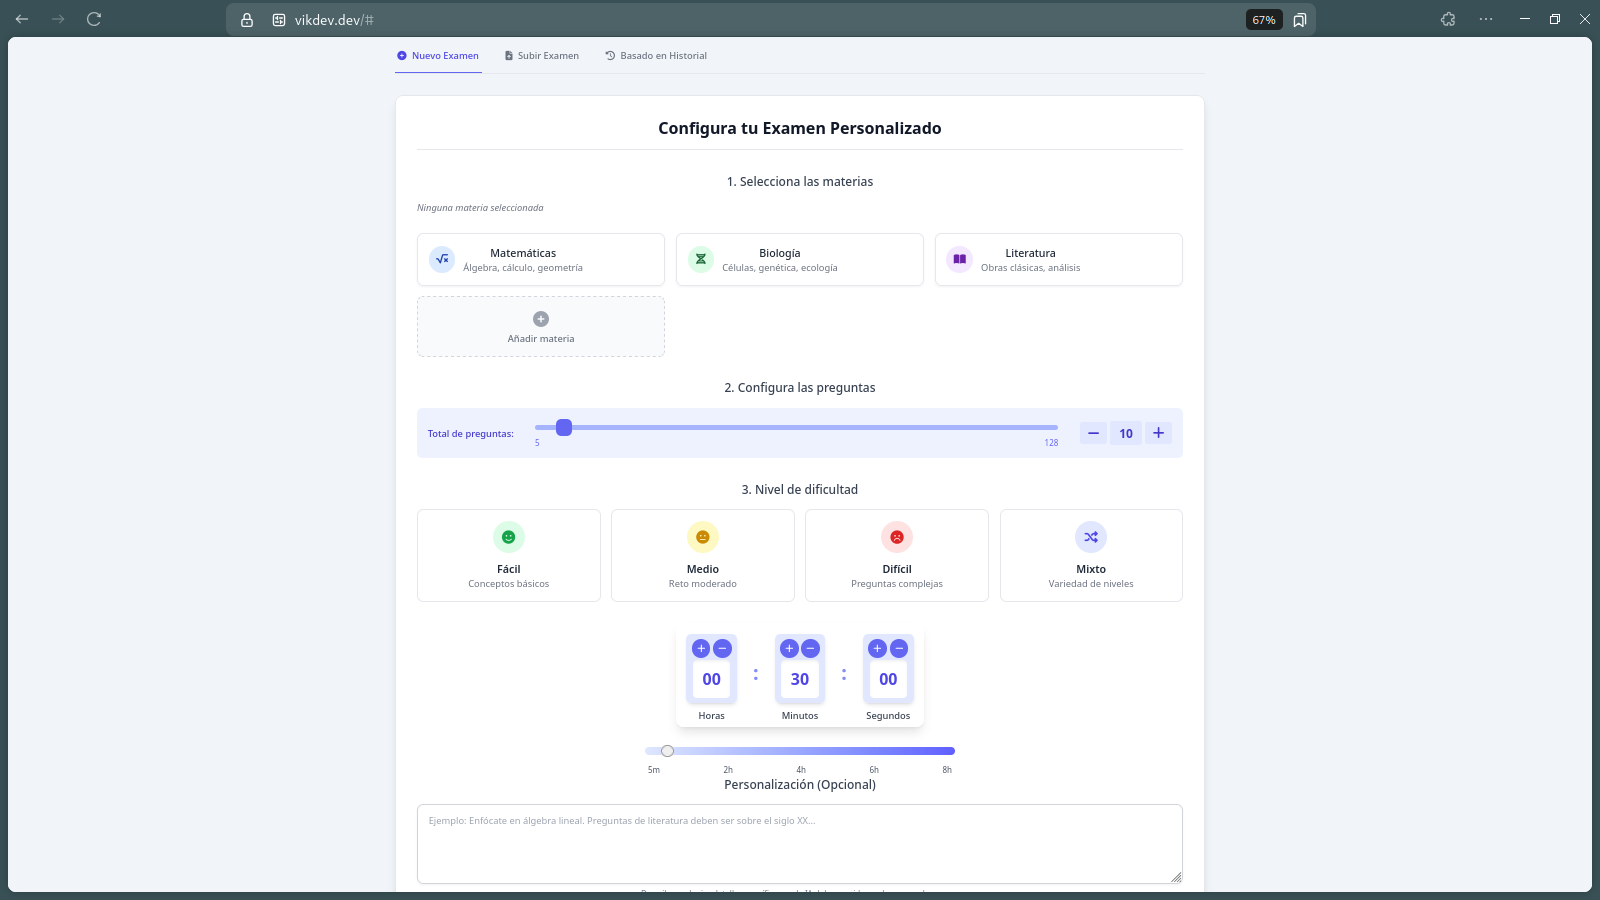
\includegraphics[width=0.9\textwidth]{250617_06h45m25s_screenshot.png}
\caption{Configuración Avanzada de Exámenes Personalizados}
\label{fig:configuracion_avanzada}
\end{figure}

\begin{figure}[h]
\centering
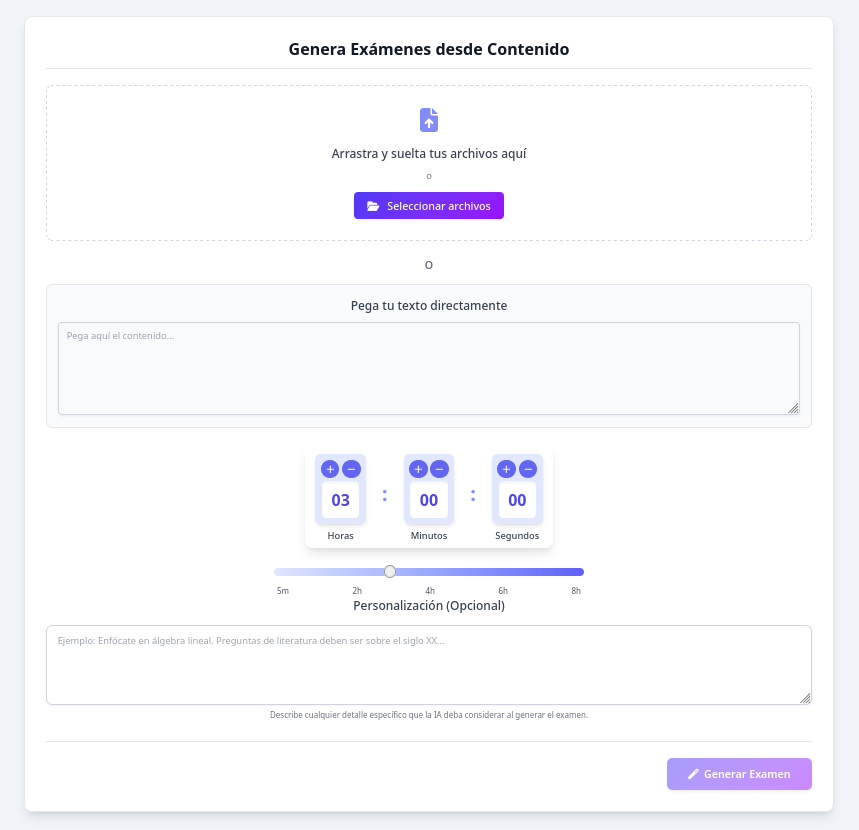
\includegraphics[width=0.9\textwidth]{250617_06h45m50s_screenshot.png}
\caption{Generación de Exámenes desde Contenido}
\label{fig:generacion_contenido}
\end{figure}

\begin{figure}[h]
\centering

\includegraphics[width=0.9\textwidth]{250617_06h46m12s_screenshot.png}
\caption{Configuración de Exámenes Basados en Historial}
\label{fig:configuracion_historial}
\end{figure}

\section{Sistema de Retroalimentación}

\subsection{Funcionalidades Avanzadas}

\subsubsection{Análisis de Respuestas}
\begin{itemize}
    \item \textbf{Evaluación automática}: Calificación instantánea
    \item \textbf{Explicaciones detalladas}: Para cada respuesta incorrecta
    \item \textbf{Sugerencias de mejora}: Areas de estudio recomendadas
    \item \textbf{Recursos adicionales}: Enlaces y materiales de apoyo
\end{itemize}

\subsubsection{Reportes Personalizados}
\begin{itemize}
    \item Análisis de fortalezas y debilidades
    \item Comparación con examenes anteriores
    \item Tendencias de aprendizaje
    \item Recomendaciones personalizadas
\end{itemize}

\subsection{Generación de Feedback con IA}

\begin{lstlisting}
const generateFeedback = async (examenId) => {
  const prompt = `
    Analiza los resultados del examen y genera:
    1. Resumen de desempeno
    2. Areas de mejora
    3. Fortalezas identificadas
    4. Plan de estudio sugerido
  `;
  
  const result = await model.generateContent(prompt);
  return result.response.text();
};
\end{lstlisting}

\subsection{Gestión de Exámenes}

\subsubsection{Lista de Exámenes Recientes}
El sistema mantiene un historial completo de todos los exámenes realizados por el usuario:

\begin{figure}[h]
\centering
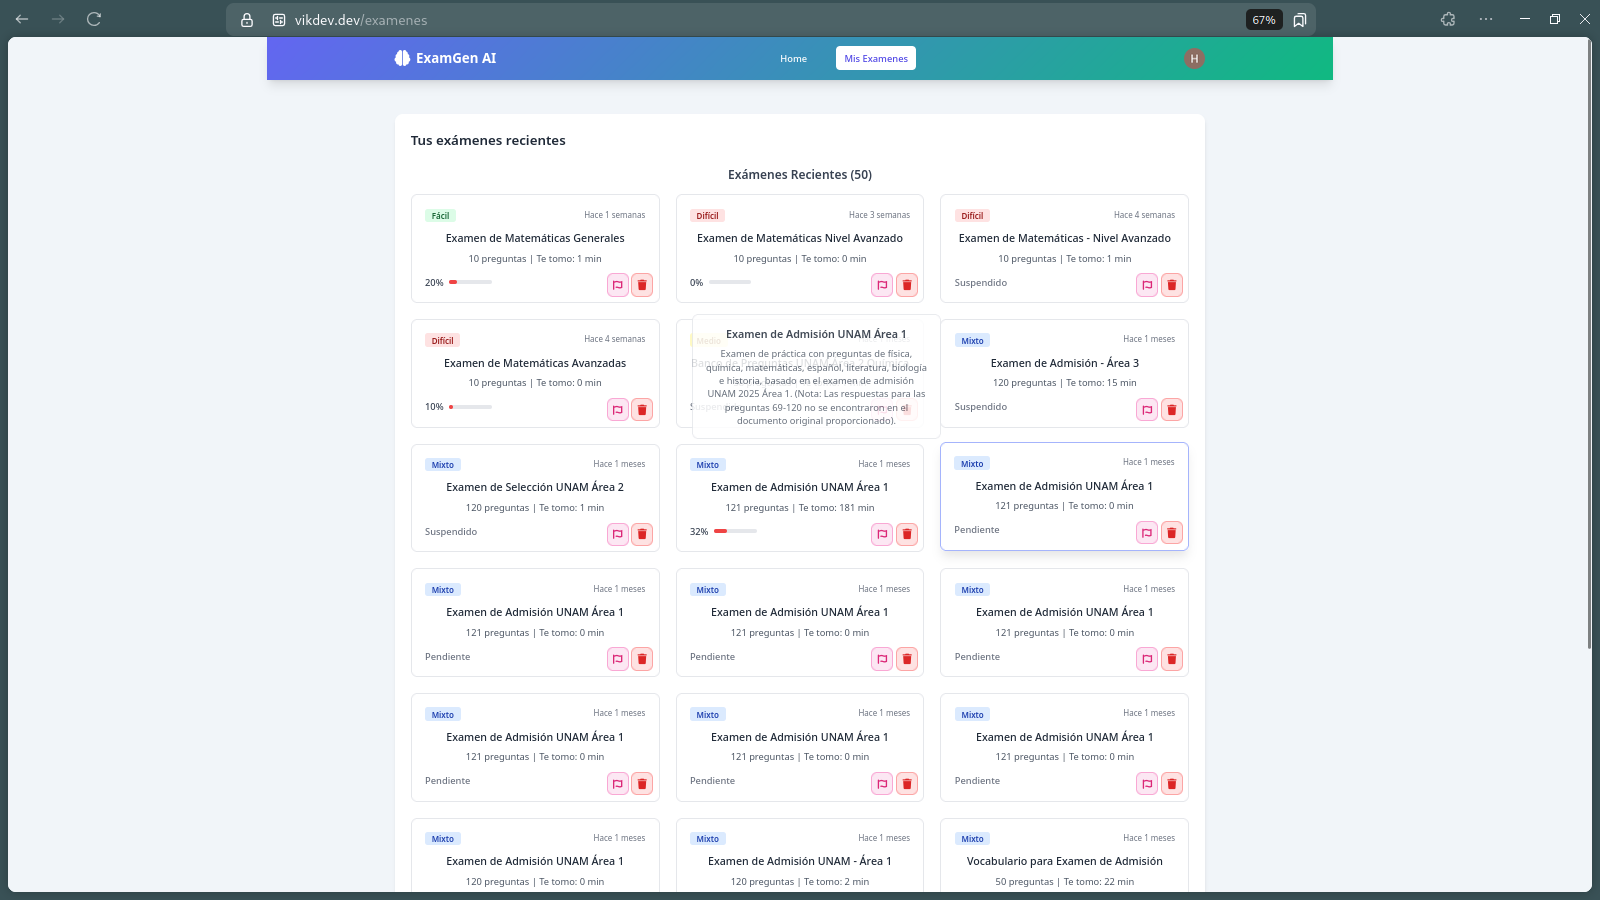
\includegraphics[width=0.9\textwidth]{250617_06h46m40s_screenshot.png}
\caption{Lista de Exámenes Recientes del Usuario}
\label{fig:examenes_recientes}
\end{figure}

\subsubsection{Interfaz de Examen en Ejecución}
Durante la realización del examen, la interfaz proporciona herramientas avanzadas de navegación:

\begin{figure}[h]
\centering

\includegraphics[width=0.9\textwidth]{250617_06h47m02s_screenshot.png}
\caption{Interfaz de Examen con Navegador de Preguntas}
\label{fig:examen_navegacion}
\end{figure}

\begin{figure}[h]
\centering

\includegraphics[width=0.9\textwidth]{250617_06h47m26s_screenshot.png}
\caption{Vista Detallada de Preguntas con Opciones Múltiples}
\label{fig:preguntas_detalle}
\end{figure}

\subsubsection{Progreso y Seguimiento}
El sistema incluye una vista completa del progreso durante el examen:

\begin{figure}[h]
\centering
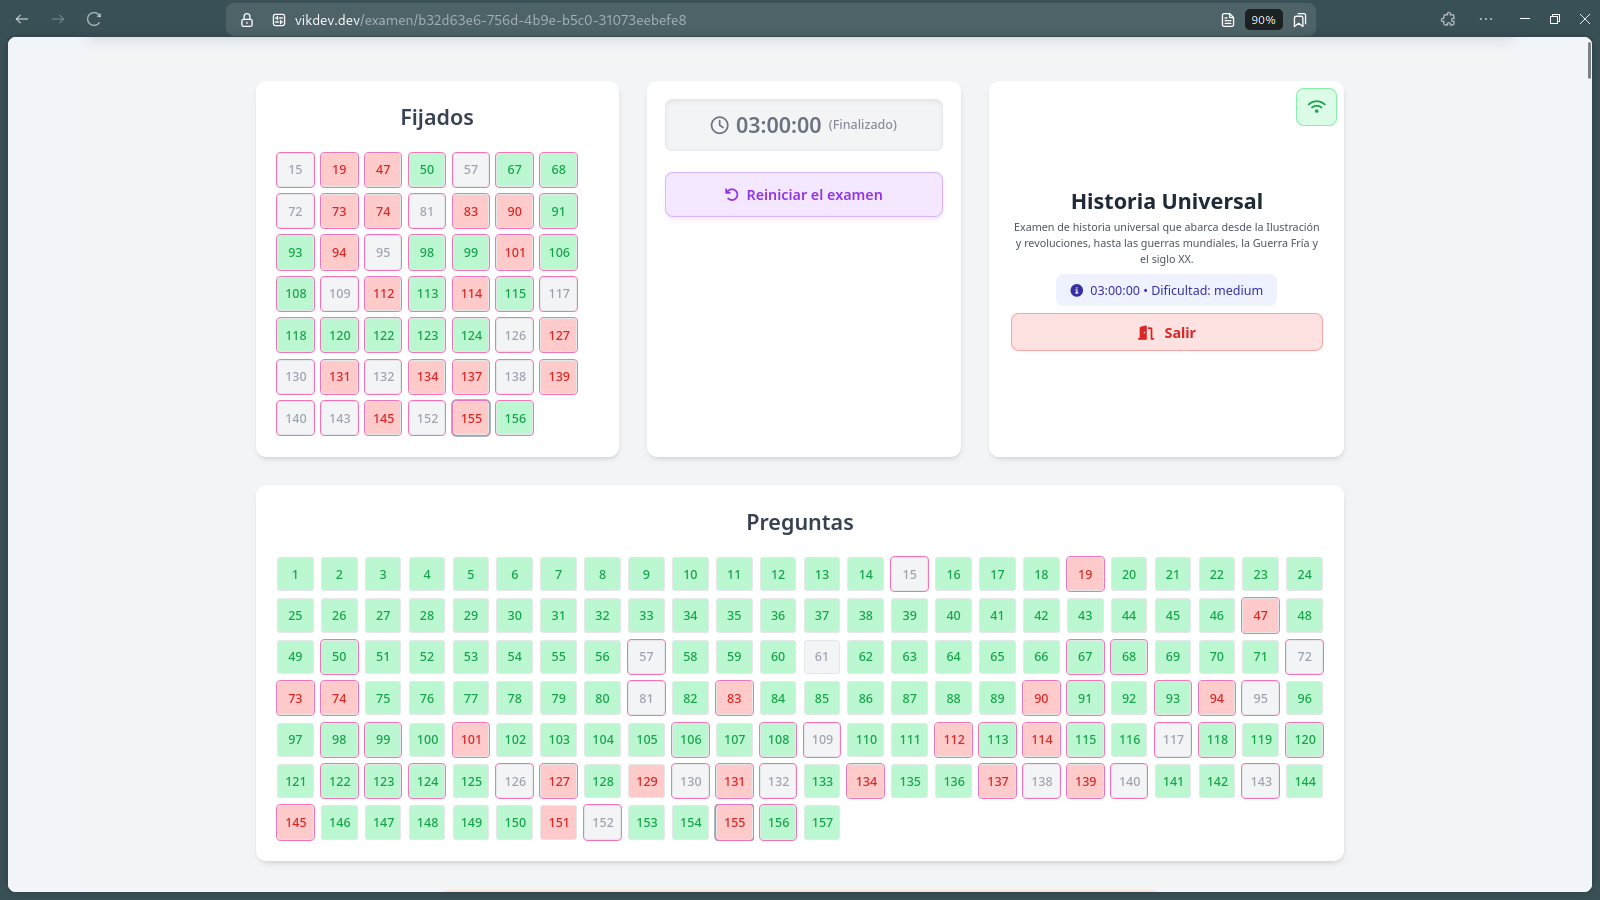
\includegraphics[width=0.9\textwidth]{250617_06h48m58s_screenshot.png}
\caption{Vista de Progreso y Estado del Examen}
\label{fig:progreso_examen}
\end{figure}

\begin{figure}[h]
\centering

\includegraphics[width=0.9\textwidth]{250617_06h49m09s_screenshot.png}
\caption{Visualización de Respuestas y Retroalimentación}
\label{fig:respuestas_feedback}
\end{figure}

\subsubsection{Finalización del Examen}
Al completar el examen, el usuario recibe opciones para revisar y obtener retroalimentación:

\begin{figure}[h]
\centering

\includegraphics[width=0.7\textwidth]{250617_06h49m37s_screenshot.png}
\caption{Pantalla de Finalización del Examen}
\label{fig:finalizacion_examen}
\end{figure}

\chapter{Configuración y Desarrollo}

\section{Requisitos del Sistema}

\subsection{Entorno de Desarrollo}

\subsubsection{Requisitos Mínimos}
\begin{itemize}
    \item \textbf{Node.js}: Versión 18 o superior
    \item \textbf{npm}: Versión 8 o superior (incluido con Node.js)
    \item \textbf{Git}: Para control de versiones
    \item \textbf{Editor de código}: VSCode recomendado
    \item \textbf{Navegador}: Chrome, Firefox o Safari actualizado
\end{itemize}

\subsubsection{Herramientas Adicionales}
\begin{itemize}
    \item \textbf{Postman}: Para pruebas de API
    \item \textbf{Chrome DevTools}: Para debugging del frontend
    \item \textbf{Supabase CLI}: Para gestión de base de datos
    \item \textbf{Flutter SDK}: Para el wrapper móvil
\end{itemize}

\subsection{Variables de Entorno}

\subsubsection{Frontend (.env)}
\begin{lstlisting}
# Configuracion de Supabase
VITE_SUPABASE_URL=https://tu-proyecto.supabase.co
VITE_SUPABASE_ANON_KEY=tu_clave_anonima

# URL del backend
VITE_BACKEND_URL=http://localhost:3001

# Configuracion de desarrollo
VITE_APP_ENV=development
VITE_DEBUG_MODE=true
\end{lstlisting}

\subsubsection{Backend (.env)}
\begin{lstlisting}
# API Key de Google Gemini
GEMINI_API_KEY=tu_api_key_de_gemini

# Configuracion de Supabase
SUPABASE_URL=https://tu-proyecto.supabase.co
SUPABASE_SERVICE_ROLE_KEY=tu_service_role_key

# Configuracion del servidor
PORT=3001
NODE_ENV=development

# Configuracion de CORS
CORS_ORIGIN=http://localhost:5173
\end{lstlisting}

\section{Dependencias del Proyecto}

\subsection{Dependencias de Producción}

\subsubsection{Frontend}
\begin{lstlisting}
{
  "dependencies": {
    "react": "^19.0.0",
    "react-dom": "^19.0.0",
    "react-router-dom": "^6.8.0",
    "@supabase/supabase-js": "^2.38.0",
    "framer-motion": "^10.16.4",
    "sweetalert2": "^11.7.32",
    "react-markdown": "^8.0.7",
    "katex": "^0.16.8",
    "react-katex": "^3.0.1"
  }
}
\end{lstlisting}

\subsubsection{Backend}
\begin{lstlisting}
{
  "dependencies": {
    "express": "^4.18.2",
    "@google/generative-ai": "^0.1.3",
    "@supabase/supabase-js": "^2.38.0",
    "multer": "^1.4.5-lts.1",
    "cors": "^2.8.5",
    "dotenv": "^16.3.1"
  }
}
\end{lstlisting}

\subsection{Dependencias de Desarrollo}

\begin{lstlisting}
{
  "devDependencies": {
    "@types/react": "^18.2.37",
    "@types/react-dom": "^18.2.15",
    "@vitejs/plugin-react": "^4.1.0",
    "vite": "^4.5.0",
    "tailwindcss": "^3.3.0",
    "autoprefixer": "^10.4.16",
    "postcss": "^8.4.31",
    "eslint": "^8.53.0",
    "prettier": "^3.0.3"
  }
}
\end{lstlisting}

\section{Proceso de Build}

\subsection{Comandos de Desarrollo}

\subsubsection{Instalación}
\begin{lstlisting}
# Clonar el repositorio
git clone https://github.com/tu-usuario/reacti.git
cd reacti

# Instalar dependencias del frontend
cd frontend
npm install

# Instalar dependencias del backend
cd ../backend
npm install
\end{lstlisting}

\subsubsection{Ejecución en Desarrollo}
\begin{lstlisting}
# Terminal 1: Ejecutar backend
cd backend
npm start

# Terminal 2: Ejecutar frontend
cd frontend
npm run dev
\end{lstlisting}

\subsection{Build de Producción}

\subsubsection{Frontend}
\begin{lstlisting}
# Generar build optimizado
cd frontend
npm run build

# El directorio 'dist' contiene los archivos optimizados
ls dist/
\end{lstlisting}

\subsubsection{Backend}
\begin{lstlisting}
# Configurar variables de entorno de produccion
export NODE_ENV=production
export PORT=3001

# Ejecutar en produccion
node src/index.js
\end{lstlisting}

\chapter{Backend y Base de Datos}

\section{Supabase como Backend}

\subsection{Componentes de Supabase}

Supabase proporciona una solución completa de Backend-as-a-Service:

\subsubsection{Base de Datos PostgreSQL}
\begin{itemize}
    \item \textbf{Esquema relacional}: Tablas optimizadas para el dominio
    \item \textbf{Índices}: Para consultas eficientes
    \item \textbf{Triggers}: Para lógica automática
    \item \textbf{Functions}: Procedimientos almacenados
\end{itemize}

\subsubsection{Autenticación}
\begin{itemize}
    \item \textbf{JWT Tokens}: Autenticación segura
    \item \textbf{Row Level Security}: Políticas de acceso granular
    \item \textbf{Providers sociales}: Login con Google, GitHub, etc.
    \item \textbf{Gestión de sesiones}: Manejo automático de tokens
\end{itemize}

\subsubsection{API REST Automática}
\begin{itemize}
    \item \textbf{CRUD operations}: Operaciones automáticas
    \item \textbf{Filtros avanzados}: Consultas complejas
    \item \textbf{Paginación}: Para grandes conjuntos de datos
    \item \textbf{Ordenamiento}: Múltiples criterios
\end{itemize}

\subsection{Estructura de la Base de Datos}

\subsubsection{Tabla: users}
\begin{lstlisting}
CREATE TABLE public.users (
    id UUID DEFAULT gen_random_uuid() PRIMARY KEY,
    email VARCHAR(255) UNIQUE NOT NULL,
    full_name VARCHAR(255),
    avatar_url TEXT,
    created_at TIMESTAMP DEFAULT NOW(),
    updated_at TIMESTAMP DEFAULT NOW()
);
\end{lstlisting}

\subsubsection{Tabla: exams}
\begin{lstlisting}
CREATE TABLE public.exams (
    id UUID DEFAULT gen_random_uuid() PRIMARY KEY,
    user_id UUID REFERENCES public.users(id) ON DELETE CASCADE,
    titulo VARCHAR(500) NOT NULL,
    descripcion TEXT,
    preguntas JSONB NOT NULL,
    dificultad VARCHAR(50) DEFAULT 'medium',
    numero_preguntas INTEGER DEFAULT 5,
    tiempo_limite INTEGER DEFAULT 1800,
    created_at TIMESTAMP DEFAULT NOW(),
    updated_at TIMESTAMP DEFAULT NOW()
);

-- Indice para busquedas por usuario
CREATE INDEX idx_exams_user_id ON public.exams(user_id);
-- Indice para busquedas por fecha
CREATE INDEX idx_exams_created_at ON public.exams(created_at);
\end{lstlisting}

\subsubsection{Tabla: exam\_results}
\begin{lstlisting}
CREATE TABLE public.exam_results (
    id UUID DEFAULT gen_random_uuid() PRIMARY KEY,
    exam_id UUID REFERENCES public.exams(id) ON DELETE CASCADE,
    user_id UUID REFERENCES public.users(id) ON DELETE CASCADE,
    respuestas JSONB NOT NULL,
    puntaje INTEGER NOT NULL DEFAULT 0,
    puntaje_maximo INTEGER NOT NULL DEFAULT 100,
    tiempo_empleado INTEGER, -- en segundos
    completed_at TIMESTAMP DEFAULT NOW(),
    
    UNIQUE(exam_id, user_id) -- Un usuario solo puede hacer un examen una vez
);
\end{lstlisting}

\subsubsection{Tabla: feedback}
\begin{lstlisting}
CREATE TABLE public.feedback (
    id UUID DEFAULT gen_random_uuid() PRIMARY KEY,
    exam_result_id UUID REFERENCES public.exam_results(id) ON DELETE CASCADE,
    user_id UUID REFERENCES public.users(id) ON DELETE CASCADE,
    feedback_data JSONB NOT NULL,
    ai_analysis TEXT,
    recommendations TEXT[],
    created_at TIMESTAMP DEFAULT NOW()
);
\end{lstlisting}

\subsection{Políticas de Seguridad}

\subsubsection{Row Level Security (RLS)}
\begin{lstlisting}
-- Habilitar RLS en todas las tablas
ALTER TABLE public.users ENABLE ROW LEVEL SECURITY;
ALTER TABLE public.exams ENABLE ROW LEVEL SECURITY;
ALTER TABLE public.exam_results ENABLE ROW LEVEL SECURITY;
ALTER TABLE public.feedback ENABLE ROW LEVEL SECURITY;

-- Politica para que usuarios solo vean sus propios datos
CREATE POLICY "Users can view own data" ON public.users
    FOR ALL USING (auth.uid() = id);

CREATE POLICY "Users can manage own exams" ON public.exams
    FOR ALL USING (auth.uid() = user_id);

CREATE POLICY "Users can view own results" ON public.exam_results
    FOR ALL USING (auth.uid() = user_id);

CREATE POLICY "Users can view own feedback" ON public.feedback
    FOR ALL USING (auth.uid() = user_id);
\end{lstlisting}

\section{Integración con Google Gemini}

\subsection{Configuración del Modelo}

\subsubsection{Inicialización del Cliente}
\begin{lstlisting}
import { GoogleGenerativeAI } from "@google/generative-ai";

class GeminiService {
    constructor() {
        this.genAI = new GoogleGenerativeAI(process.env.GEMINI_API_KEY);
        this.modelFlash = this.genAI.getGenerativeModel({
            model: "gemini-2.0-flash"
        });
        this.modelPro = this.genAI.getGenerativeModel({
            model: "gemini-2.5-pro-exp-03-25"
        });
    }
    
    async generateExam(content, difficulty = 'medium') {
        const model = difficulty === 'hard' ? this.modelPro : this.modelFlash;
        const prompt = this.buildExamPrompt(content, difficulty);
        
        try {
            const result = await model.generateContent(prompt);
            return this.parseExamResponse(result.response.text());
        } catch (error) {
            throw new Error(`Error generando examen: ${error.message}`);
        }
    }
}
\end{lstlisting}

\subsection{Funcionalidades de IA}

\subsubsection{Generación de Preguntas}
\begin{lstlisting}
buildExamPrompt(content, difficulty) {
    return `
        Analiza el siguiente contenido y crea un examen con estas especificaciones:
        
        Contenido: ${content}
        Dificultad: ${difficulty}
        
        Genera un JSON con la siguiente estructura:
        {
            "titulo": "Titulo del examen",
            "descripcion": "Descripcion breve",
            "numero_preguntas": 5,
            "dificultad": "${difficulty}",
            "preguntas": [
                {
                    "id": 1,
                    "pregunta": "Texto de la pregunta",
                    "opciones": ["opcion1", "opcion2", "opcion3", "opcion4"],
                    "correcta": 0,
                    "explicacion": "Explicacion de la respuesta correcta"
                }
            ]
        }
        
        Asegurate de que las preguntas sean relevantes y del nivel solicitado.
    `;
}
\end{lstlisting}

\subsubsection{Análisis de Resultados}
\begin{lstlisting}
async generateFeedback(examResult) {
    const prompt = `
        Analiza los resultados de este examen y proporciona feedback personalizado:
        
        Puntaje obtenido: ${examResult.puntaje}/${examResult.puntaje_maximo}
        Tiempo empleado: ${examResult.tiempo_empleado} segundos
        Respuestas: ${JSON.stringify(examResult.respuestas)}
        
        Genera un analisis que incluya:
        1. Resumen del desempeno
        2. Fortalezas identificadas
        3. Areas de mejora
        4. Recomendaciones especificas de estudio
        5. Proximos pasos sugeridos
        
        El feedback debe ser constructivo y motivador.
    `;
    
    const result = await this.modelPro.generateContent(prompt);
    return result.response.text();
}
\end{lstlisting}

\chapter{API Endpoints y Comunicación}

\section{Endpoints de Autenticación}

\subsection{Registro de Usuario}
\begin{lstlisting}
POST /api/auth/register
Content-Type: application/json

{
    "email": "usuario@ejemplo.com",
    "password": "password123",
    "full_name": "Nombre Completo"
}

Response:
{
    "success": true,
    "user": {
        "id": "uuid",
        "email": "usuario@ejemplo.com",
        "full_name": "Nombre Completo"
    },
    "token": "jwt_token"
}
\end{lstlisting}

\subsection{Inicio de Sesión}
\begin{lstlisting}
POST /api/auth/login
Content-Type: application/json

{
    "email": "usuario@ejemplo.com",
    "password": "password123"
}

Response:
{
    "success": true,
    "user": { ... },
    "token": "jwt_token"
}
\end{lstlisting}

\section{Endpoints de Examenes}

\subsection{Generar Examen desde Archivo}
\begin{lstlisting}
POST /api/upload_files
Authorization: Bearer jwt_token
Content-Type: multipart/form-data

Files: archivo.pdf
Body:
{
    "prompt": "Genera preguntas sobre este documento",
    "tiempo_limite_segundos": 1800,
    "numero_preguntas": 10,
    "dificultad": "medium"
}

Response:
{
    "success": true,
    "exam": {
        "id": "uuid",
        "titulo": "Examen generado",
        "preguntas": [...],
        "tiempo_limite": 1800
    }
}
\end{lstlisting}

\subsection{Generar Examen desde Texto}
\begin{lstlisting}
POST /api/generate-content
Authorization: Bearer jwt_token
Content-Type: application/json

{
    "prompt": "Crea un examen sobre JavaScript",
    "dificultad": "medium",
    "numero_preguntas": 8,
    "tiempo_limite_segundos": 1200
}

Response:
{
    "success": true,
    "exam": { ... }
}
\end{lstlisting}

\subsection{Obtener Examenes del Usuario}
\begin{lstlisting}
GET /api/exams
Authorization: Bearer jwt_token

Response:
{
    "success": true,
    "exams": [
        {
            "id": "uuid",
            "titulo": "Examen de JavaScript",
            "created_at": "2025-06-19T10:00:00Z",
            "numero_preguntas": 10,
            "dificultad": "medium"
        }
    ]
}
\end{lstlisting}

\section{Endpoints de Resultados}

\subsection{Enviar Respuestas de Examen}
\begin{lstlisting}
POST /api/exam-results
Authorization: Bearer jwt_token
Content-Type: application/json

{
    "exam_id": "uuid",
    "respuestas": [
        {
            "pregunta_id": 1,
            "respuesta_seleccionada": 2
        }
    ],
    "tiempo_empleado": 900
}

Response:
{
    "success": true,
    "result": {
        "id": "uuid",
        "puntaje": 85,
        "puntaje_maximo": 100,
        "respuestas_correctas": 8,
        "total_preguntas": 10
    }
}
\end{lstlisting}

\subsection{Generar Retroalimentación}
\begin{lstlisting}
POST /api/generate-feedback
Authorization: Bearer jwt_token
Content-Type: application/json

{
    "exam_result_id": "uuid"
}

Response:
{
    "success": true,
    "feedback": {
        "analysis": "Analisis detallado del desempeno...",
        "strengths": ["Conceptos basicos", "Sintaxis"],
        "improvements": ["Programacion asincrona"],
        "recommendations": ["Practicar con async/await"]
    }
}
\end{lstlisting}

\chapter{Costos y Viabilidad Económica}

\section{Análisis Detallado de Costos}

El Sistema de Generación de Exámenes con IA (ExamGenAI) ha sido desarrollado con un enfoque de costos optimizados, ideal para equipos pequeños y proyectos educativos con presupuesto limitado.

\subsection{Estructura de Costos}

\subsubsection{Costos de Desarrollo}
\begin{itemize}
    \item \textbf{Tiempo de desarrollo}: 4 meses aproximadamente
    \item \textbf{Herramientas de desarrollo}: Gratuitas (VS Code, Git, etc.)
\end{itemize}

\subsubsection{Costos de Infraestructura}
\begin{table}[h]
\centering
\begin{tabular}{|l|l|r|}
\hline
\textbf{Servicio} & \textbf{Proveedor} & \textbf{Costo Mensual} \\
\hline
Base de Datos & Supabase (Tier gratuito) & \$0.00 \\
Hosting Frontend & Hostinger & \$2.99 \\
API Gemini & Google (cuota gratuita) & \$0.00 \\
Servidor Backend & VPS básico & \$5.00 \\
Dominio & Registro anual & \$1.00 \\
\hline
\textbf{Total Mensual} & & \textbf{\$8.99} \\
\hline
\end{tabular}
\caption{Desglose Completo de Costos de Infraestructura}
\end{table}

\subsubsection{Costos de Escalamiento}
\begin{itemize}
    \item \textbf{Supabase Pro}: \$25/mes (para más de 500MB de DB)
    \item \textbf{Google Gemini Pro}: \$0.002 por 1K tokens de entrada
    \item \textbf{VPS Pro}: \$20/mes (para mayor tráfico)
    \item \textbf{CDN}: \$10/mes (para distribución global)
\end{itemize}

\subsection{Ventajas del Modelo de Costos}
\begin{itemize}
    \item \textbf{Inicio gratuito}: Posible comenzar sin inversión inicial
    \item \textbf{Escalamiento gradual}: Costos crecen con el uso
    \item \textbf{Sin licencias costosas}: Tecnologías open source
    \item \textbf{Mantenimiento mínimo}: Servicios administrados
\end{itemize}

\subsection{Comparación con Alternativas}
\begin{table}[h]
\centering
\begin{tabular}{|l|r|r|r|}
\hline
\textbf{Solución} & \textbf{Costo Inicial} & \textbf{Costo Mensual} & \textbf{Costo Anual} \\
\hline
ExamGenAI & \$0 & \$8.99 & \$107.88 \\
Moodle + Hosting & \$500 & \$25.00 & \$800.00 \\
Canvas LMS & \$0 & \$50.00 & \$600.00 \\
Blackboard & \$2000 & \$100.00 & \$3200.00 \\
\hline
\end{tabular}
\caption{Comparación de Costos con Plataformas Educativas}
\end{table}

\section{Modelo de Negocio}

\subsection{Opciones de Monetización}
\begin{itemize}
    \item \textbf{Freemium}: Versión básica gratuita, funciones avanzadas de pago
    \item \textbf{Suscripción institucional}: Planes para escuelas y universidades
    \item \textbf{API como servicio}: Integración con otras plataformas
    \item \textbf{Consultoría}: Implementación personalizada
\end{itemize}

\subsection{Proyección de Ingresos}
\begin{table}[h]
\centering
\begin{tabular}{|l|r|r|r|}
\hline
\textbf{Plan} & \textbf{Precio Mensual} & \textbf{Usuarios Objetivo} & \textbf{Ingreso Mensual} \\
\hline
Básico & \$0 & 1000 & \$0 \\
Pro & \$9.99 & 100 & \$999 \\
Institucional & \$49.99 & 20 & \$999.80 \\
Enterprise & \$199.99 & 5 & \$999.95 \\
\hline
\textbf{Total Proyectado} & & \textbf{1125} & \textbf{\$2998.75} \\
\hline
\end{tabular}
\caption{Proyección de Ingresos Mensuales}
\end{table}

\chapter{Seguridad y Optimización}

\section{Medidas de Seguridad}

\subsection{Autenticación y Autorización}
\begin{itemize}
    \item \textbf{JWT Tokens}: Tokens seguros con expiración
    \item \textbf{Validación de entrada}: Sanitización de datos
    \item \textbf{Rate limiting}: Límites de peticiones por IP
    \item \textbf{CORS configurado}: Solo orígenes permitidos
\end{itemize}

\subsection{Protección de Datos}
\begin{itemize}
    \item \textbf{Encriptación en tránsito}: HTTPS obligatorio
    \item \textbf{Variables de entorno}: Credenciales seguras
    \item \textbf{Row Level Security}: Políticas de acceso granular
    \item \textbf{Limpieza de archivos}: Eliminación automática de temporales
\end{itemize}

\section{Optimización de Rendimiento}

\subsection{Frontend}
\begin{itemize}
    \item \textbf{Lazy loading}: Carga bajo demanda de componentes
    \item \textbf{Memoización}: Evitar re-renders innecesarios
    \item \textbf{Bundle splitting}: Código dividido por rutas
    \item \textbf{Compresión}: Assets optimizados para producción
\end{itemize}

\subsection{Backend}
\begin{itemize}
    \item \textbf{Conexión pool}: Reutilización de conexiones DB
    \item \textbf{Caché}: Resultados frecuentes en memoria
    \item \textbf{Compresión gzip}: Respuestas comprimidas
    \item \textbf{Índices de BD}: Consultas optimizadas
\end{itemize}

\chapter{Despliegue, Monitoreo y Mantenimiento}

\section{Proceso de Despliegue}

\subsection{Frontend (Hostinger)}
\begin{lstlisting}
# 1. Generar build de produccion
npm run build

# 2. Configurar variables de entorno de produccion
VITE_SUPABASE_URL=https://prod.supabase.co
VITE_BACKEND_URL=https://api.reacti.com

# 3. Subir archivos a hosting
# Copiar contenido de 'dist' al directorio public_html
\end{lstlisting}

\subsection{Backend (Servidor VPS)}
\begin{lstlisting}
# 1. Clonar repositorio en servidor
git clone https://github.com/usuario/reacti.git
cd reacti/backend

# 2. Instalar dependencias
npm install --production

# 3. Configurar variables de entorno
export NODE_ENV=production
export GEMINI_API_KEY=tu_api_key
export SUPABASE_URL=https://prod.supabase.co

# 4. Ejecutar con PM2
pm2 start src/index.js --name "reacti-api"
pm2 save
pm2 startup
\end{lstlisting}

\chapter{Exposición Móvil con Flutter WebView}
\label{chap:flutter_webview}

Para expandir el alcance de la plataforma ExamGenAI a dispositivos móviles de manera rápida y eficiente, se adoptó la estrategia de encapsular la aplicación web existente dentro de un contenedor móvil. La tecnología elegida para esta tarea fue Flutter, debido a su naturaleza multiplataforma y su facilidad para integrar WebViews.

\section{Estrategia y Justificación}

La adopción de un enfoque de WebView, en lugar de desarrollar una aplicación nativa desde cero, se basó en las siguientes consideraciones clave:

\begin{itemize}
    \item \textbf{Rapidez de lanzamiento (Time-to-Market):} Permitió tener una versión móvil funcional en una fracción del tiempo que tomaría un desarrollo nativo completo.
    \item \textbf{Reutilización del código:} Se aprovecha el 100\% del frontend desarrollado en React, incluyendo toda la lógica, componentes y comunicación con el backend.
    \item \textbf{Mantenimiento centralizado:} Cualquier actualización en la aplicación web se refleja inmediatamente en la aplicación móvil, sin necesidad de publicar una nueva versión en las tiendas.
    \item \textbf{Costo-efectividad:} Minimiza los costos de desarrollo al no requerir un equipo de desarrollo móvil dedicado.
\end{itemize}

\section{Implementación Técnica}

El núcleo de la aplicación móvil es el paquete \texttt{webview\_flutter}. La implementación consiste en una aplicación de Flutter mínima cuya pantalla principal es un widget \texttt{WebViewWidget} que carga la URL de producción del frontend.

\begin{lstlisting}[language=Dart, caption={Implementación básica del WebView en Flutter}]
import 'package:flutter/material.dart';
import 'package:webview_flutter/webview_flutter.dart';

void main() {
  runApp(const MyApp());
}

class MyApp extends StatelessWidget {
  const MyApp({super.key});

  @override
  Widget build(BuildContext context) {
    return MaterialApp(
      title: 'ExamGenAI',
      theme: ThemeData(
        primarySwatch: Colors.blue,
        useMaterial3: true,
      ),
      home: const WebViewPage(),
      debugShowCheckedModeBanner: false,
    );
  }
}

class WebViewPage extends StatefulWidget {
  const WebViewPage({super.key});

  @override
  State<WebViewPage> createState() => _WebViewPageState();
}

class _WebViewPageState extends State<WebViewPage> {
  late final WebViewController _controller;
  bool _isLoading = true;

  @override
  void initState() {
    super.initState();
    _controller = WebViewController()
      ..setJavaScriptMode(JavaScriptMode.unrestricted)
      ..setNavigationDelegate(
        NavigationDelegate(
          onPageStarted: (String url) {
            setState(() {
              _isLoading = true;
            });
          },
          onPageFinished: (String url) {
            setState(() {
              _isLoading = false;
            });
          },
        ),
      )
      ..loadRequest(Uri.parse('https://vikdev.dev/')); // URL de Producción
  }

  @override
  Widget build(BuildContext context) {
    return Scaffold(
      body: SafeArea(
        child: Stack(
          children: [
            WebViewWidget(controller: _controller),
            if (_isLoading)
              const Center(
                child: CircularProgressIndicator(),
              ),
          ],
        ),
      ),
    );
  }
}
\end{lstlisting}

\section{Ventajas y Limitaciones de la Estrategia}

\subsubsection{Ventajas}
\begin{itemize}
    \item \textbf{Desarrollo acelerado:} La principal ventaja es la velocidad de implementación.
    \item \textbf{Experiencia de usuario consistente:} La interfaz es idéntica en la web y en el móvil.
    \item \textbf{Un solo codebase para la UI/UX:} Reduce la complejidad del proyecto.
\end{itemize}

\subsubsection{Limitaciones}
\begin{itemize}
    \item \textbf{Rendimiento:} El rendimiento puede no ser tan fluido como una aplicación nativa.
    \item \textbf{Dependencia de la conexión:} La aplicación requiere una conexión a internet constante.
    \item \textbf{Dificultad con flujos complejos:} Flujos de autenticación de terceros (OAuth) son problemáticos de implementar y a menudo son bloqueados por los proveedores por seguridad, requiriendo soluciones más complejas.
    \item \textbf{Acceso limitado a APIs nativas:} El acceso a hardware del dispositivo (cámara, GPS, etc.) es limitado.
\end{itemize}

\chapter{Conclusión}

\section{Resumen del Sistema}

El Sistema de Generación de Examenes con IA (ExamGenAI) representa una solución moderna y escalable para la automatización de evaluaciones educativas. Utilizando tecnologías de vanguardia como React, Node.js, y Supabase, el sistema proporciona una experiencia web completa, extendida a dispositivos móviles a través de un wrapper básico con Flutter.

\subsection{Características Principales}
\begin{itemize}
    \item \textbf{Generación automática}: Preguntas basadas en documentos o texto libre.
    \item \textbf{Múltiples dificultades}: Adaptación automática del nivel.
    \item \textbf{Retroalimentación IA}: Análisis detallado del desempeño.
    \item \textbf{Interfaz moderna}: Diseño responsive y accesible.
    \item \textbf{Seguridad robusta}: Protección de datos y autenticación segura.
    \item \textbf{Acceso multiplataforma}: Disponible en la web y como aplicación móvil (iOS/Android) a través de un WebView.
\end{itemize}

\subsection{Beneficios Técnicos}
\begin{itemize}
    \item \textbf{Arquitectura escalable}: Fácil mantenimiento y extensión.
    \item \textbf{Tecnologías modernas}: Stack actualizado y soporte a largo plazo.
    \item \textbf{Base de datos optimizada}: Consultas eficientes y seguras.
    \item \textbf{API bien diseñada}: Endpoints claros y documentados.
\end{itemize}

\section{Trabajo Futuro}

El enfoque futuro del proyecto se centra en la expansión de funcionalidades y la optimización de la infraestructura para un crecimiento sostenido.

\subsection{Mejoras Planificadas}
\begin{itemize}
    \item \textbf{Soporte multiidioma}: Internacionalización completa de la plataforma.
    \item \textbf{Análisis avanzado}: Incorporar métricas de aprendizaje más sofisticadas y reportes visuales.
    \item \textbf{Integración con LMS}: Desarrollar compatibilidad con sistemas de gestión de aprendizaje (LMS) como Moodle o Canvas.
    \item \textbf{App móvil nativa}: Evolucionar el actual wrapper de WebView a una aplicación completamente nativa (en Flutter o nativo) para mejorar el rendimiento, habilitar funciones offline y permitir una integración robusta con flujos de autenticación de terceros y APIs del dispositivo.
\end{itemize}

\subsection{Escalabilidad}
\begin{itemize}
    \item \textbf{Microservicios}: Migración gradual del backend a una arquitectura de microservicios.
    \item \textbf{Cache distribuido}: Implementación de Redis para almacenar en caché resultados de API frecuentes.
    \item \textbf{CDN (Content Delivery Network)}: Uso de una CDN para distribuir globalmente los assets del frontend.
    \item \textbf{Auto-scaling}: Configuración de la infraestructura del backend para escalar automáticamente según la demanda.
\end{itemize}

\vspace{2cm}

\noindent\textbf{Versión del Manual}: 1.0\\
\textbf{Fecha}: 19 de junio de 2025\\
\textbf{Desarrollado por}: Hernández Tellez Héctor Fidel, Rivero Flores Victor Gabriel

\end{document}
